\documentclass[pageno]{jpaper}

%replace XXX with the submission number you are given from the ASPLOS submission site.
\newcommand{\asplossubmissionnumber}{127}

\usepackage{times}
\usepackage{datetime}
\usepackage{balance}  % to better equalize the last page
\usepackage{graphics} % for EPS, load graphicx instead
\usepackage{url}
\usepackage{hyperref}
\usepackage{txfonts}
\usepackage{pslatex}    
\usepackage{pifont}
%\usepackage{bbding}
\usepackage{multirow}
\usepackage{makecell}
\usepackage[justification=centering]{caption}
\usepackage{xspace}
\usepackage{comment}
\usepackage{listings}
%\usepackage[section]{placeins}
\usepackage{tikz}
\usepackage{calc}
\usepackage{fancyvrb}
\usepackage{xcolor}
\usepackage{flushend}
\usepackage{wrapfig}

\newcommand{\cmark}{\ding{51}}%
\newcommand{\xmark}{\ding{55}}%

\newcommand{\eurosyssubmissionnumber}{\#147, 12 pages}
\newcommand{\todo}[1]{{\color{red}\bfseries [[#1]]}}
\newcommand{\TP}[1]{{\color{red}\bfseries [[#1]]}}

\newcommand{\specialcell}[2][c]{%
  \begin{tabular}[#1]{@{}c@{}}#2\end{tabular}}
\newcommand{\OB}{\texttt{OpenBSD}}
\newcommand{\DieHarder}{\texttt{DieHarder}}
\newcommand{\DL}{\texttt{DLmalloc}}
\newcommand{\JE}{\texttt{jemalloc}}
\newcommand{\MP}{\texttt{mmprof}}
\newcommand{\RN}[1]{\uppercase\expandafter{\romannumeral #1\relax}}


\begin{document}

\title{mmprof: A General Profiler for Different Memory Allocators\\ \textbf{Extended Abstract}}

\date{}

\maketitle

% No abstract needed for the extended abstract
%\begin{abstract}
%\end{abstract}


\section{Motivation}
\label{sec:motivation}

A memory allocator is a key component that could significantly impact the performance and memory consumption of the corresponding applications by up to orders of magnitude. However, none of existing tools could answer the following questions related to the memory allocator. \\

\begin{itemize}
\item Whether the allocator introduces   some performance slowdown for this application? 
\item How much the performance can be improved if switching to a well-performed allocator (e.g., TcMalloc)?
\item How much memory wastes the allocator introduces?
\item What are the possible design issues for performance slowdown and memory wastes separately? 
%\item What are quantitative metrics to evaluate a memory allocator? 
\end{itemize}
\vspace{0.1in}

Due to the obvious importance of a memory allocator, it is emergent to design a profiler that could answer these research questions about an allocator. This paper presents such a profiler--\MP{}--that profiles different aspects of an allocator that will benefit both allocator designers and normal users. 

\MP{} will benefit normal users by predicting potential performance impact, reporting detailed memory wastes, and judging whether an allocator is tapped with allocation/deallocation pattern or access pattern of the current application. \MP{} will also benefit allocator designers that help diagnose the specific design issues inside the allocator. 

\section{Limitations of the State of the Art}
\label{sec:limitations}

None of existing profilers can identify the inherent reasons of performance slowdown and memory wastes caused by an allocator. 

General profilers, such as \texttt{gprof}~\cite{DBLP:conf/sigplan/GrahamKM82} and \texttt{perf}~\cite{perf}, only report the time accumulation of different functions, and \texttt{Coz}~\cite{Coz} presents a quantitative performance impact of improving a particular region of code. Although they may identify some performance bottlenecks inside applications, but they could not shed light on the performance issues caused by the allocator. 

 Existing allocator profilers, such as \texttt{mprof}~\cite{Zorn:1988:MAP:894814}, Mtrace~\cite{mtrace}, Mtrace++~\cite{Lee:2000:DMM:786772.787150}, \texttt{TcMalloc} profiler~\cite{tcmalloc-profiler}, or CLR profiler~\cite{lupasc2014dynamic}, mainly focus on how an application uses the memory, but not on memory wastes caused by the allocator itself. 


\section{Key Insights}
\label{sec:key-insights}

\begin{itemize}
\item What are the one or two key new insights in this paper?
\end{itemize}

\begin{figure}[!ht]
\centering
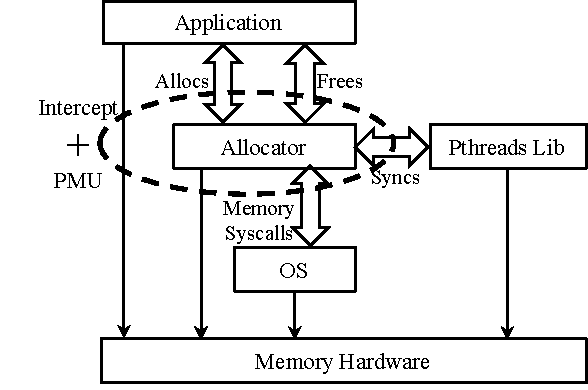
\includegraphics[width=3in]{figures/overview}
\caption{Basic idea of \texttt{mmprof}.\label{fig:basicidea}}
\end{figure}

\MP{} is designed as a drop-in library that can be simply linked to applications (and allocators) with the preloading mechanism, which does not require the change or the re-compilation of applications and allocators, as far as an allocator utilizes standard synchronizations and system calls.


\begin{itemize}
\item How does it advance the state of the art?
\end{itemize}

\noindent
Firstly, \MP{} is the first systematic approach to evaluate and profile different memory allocators, without changing the internal implementation of allocators. More specifically, \MP{} proposes the combination of function interception (based on common APIs) and PMU-based sampling to perform the profiling. Besides, \MP{} proposes the first mechanisms to quantitatively measure memory blowup (and external fragmentation), cache/page utilization rate, and passive/active false sharing impact.  

%\MP{} will benefit normal users in the following ways. First, \MP{} can predict potential performance improvement when switching to an exemplar allocator (such as TcMalloc), which clearly indicates whether it is necessary to improve the allocator or switch to a new allocator. Second, \MP{} will report detailed memory wastes caused by an allocator, which is overlooked by existing profilers. Third, \MP{} will also report multiple application-friendliness metrics, which tells whether an allocator is tapped with allocation/deallocation pattern or access pattern of a particular application. As described above, a well-performed allocator like TcMalloc may be not suitable for a particular application (e.g., \texttt{cache-thrash}). Overall, \MP{} will provide a range of metrics on evaluating an allocator for normal users, not just limiting to the runtime. 

\begin{itemize}
\item What makes it more effective than past approaches?
\end{itemize}

\begin{itemize}
\item It will quantify application-friendliness, which is not available in existing work, and which helps users to decide which allocator should be used for a specific application. 
\item It will provide the memory usage (overhead) information, such as internal fragmentation, and objects that are not freed but yet which remain unused. 
\item It will provide some information that only exists across multiple profilers, for instance, the average number of instructions of each allocation and deallocation, the average time spent within each allocation and deallocation (PMU sampling will be placed outside of the time span, thus not avoiding an erroneous measurement of how long this allocation and deallocation request has been sampled), whether there are some contentions during allocation (user space and kernel space), how many lock acquisitions.  
\end{itemize}

\section{Main Artifacts}
\label{sec:main-artifacts}

\begin{itemize}
\item What are the key artifacts presented in your paper: a
  methodology, a hardware design, a software algorithm, an
  optimization or control technique, etc.?
\end{itemize}

The key artifacts of this paper is a profiling tool that could 

\noindent
To profile an allocator, \MP{} intercepts memory allocations/deallocations, memory-related system calls, and synchronizations. This also indicates that an allocator should utilize standard APIs in order for \MP{} to collect corresponding information. However, the Linux allocator utilizes the internal implementation of synchronizations by default. For the profiling purpose, it should be changed to invoke explicit POSIX-APIs instead. Fortunately, most allocators do not need any change or the recompilation.  \MP{} profiles the performance, memory overhead, scalability, and application friendliness, as discussed in different subsections. It also discusses some common issues, such as adapting to different allocators, and the performance issue of collecting data. 

\begin{itemize}
  \item How were your artifacts implemented and evaluated? 
\end{itemize}

\noindent
\MP{} is written as a runtime library that could be attached to different allocators, as far as . 
We evaluate how \MP{} could benefit both normal users and allocator designers. 
The former includes \textbf{Prediction of Performance Improvement}, \textbf{Reporting Memory Overhead} and \textbf{Reporting Application Friendliness}. 
To evaluate the latter one, we evaluate \MP{} with five widely-used allocators, including two versions of the Linux allocator (versions 2.21 and 2.28), TCMalloc~\cite{tcmalloc}, jemalloc, and Hoard, and two secure allocators, i.e. DieHarder and OpenBSD. These allocators include both sequential and BiBOP-style allocators. Secure allocators were included, since they have their unique memory management policies. 


\section{Key Results and Contributions}
\label{sec:key-contributions}

\begin{itemize}
  \item What are the most important \emph{one or two} empirical or theoretical
    results of this approach?
\end{itemize}

\begin{itemize}
  \item What are the contributions that this paper makes to the state of the
    art? List them in an \texttt{itemize} section. Each contribution should be no more than a few sentences long.
\end{itemize}

\begin{itemize}
  \item Clearly describe its advantages over past work, including how it overcomes their limitations.
\end{itemize}


\section{Why ASPLOS}
\label{sec:why-asplos}

This paper describes a tool that could be utilized to identify .
Firstly, \MP{} is an effective tool which could help both allocator designers and normal users, so we are confident that \MP{} benefits multidisciplinary areas. Second, the paper concludes and shares core understanding of relationship between application performance and allocators, which is a basic but significant topic for multiple fields.


\section{Citation for Most Influential Paper Award}
\label{sec:citation}

Provide the citation for your paper if it won a Most Influential
Paper award. You can find example citations
on the \href{https://www.sigops.org/awards/hof/}{SIGOPS Hall of Fame}
and \href{https://www.sigplan.org/Awards/PLDI/}{PLDI most influential
  paper list}.  Limit the citation to 1-3 sentences
\emph{Recall that your citation here must be anonymous}; do not include names or affiliations.

%  \url{https://rb.gy/hd1hms}).

\section{Revisions}
\label{sec:revisions}

     a lack sufficient research novelty
    high tool overhead
    lack of portability
    many unanswered questions concerning the empirical methodology and results
    the use case for the tool is overly narrow for an OOPSLA publication.

The revision of this paper is improved in the following aspects. First, we significantly reduce its performance overhead via two approaches. First, the overhead of collecting counting events is the most significant overhead, where the overhead could be delayed to second time, where most of  sampling technique. Second, this version also strengths how \MP{} could be utilized to benefit normal users, avoiding the narrow usage issue pointed out by previous reviewers. Third, we re-write the introduction to focus more on research novelty. 
 
\pagebreak
{
\bibliographystyle{plain}
\bibliography{refs, tongping, sam}
}



\end{document}

